{
\usebackgroundtemplate{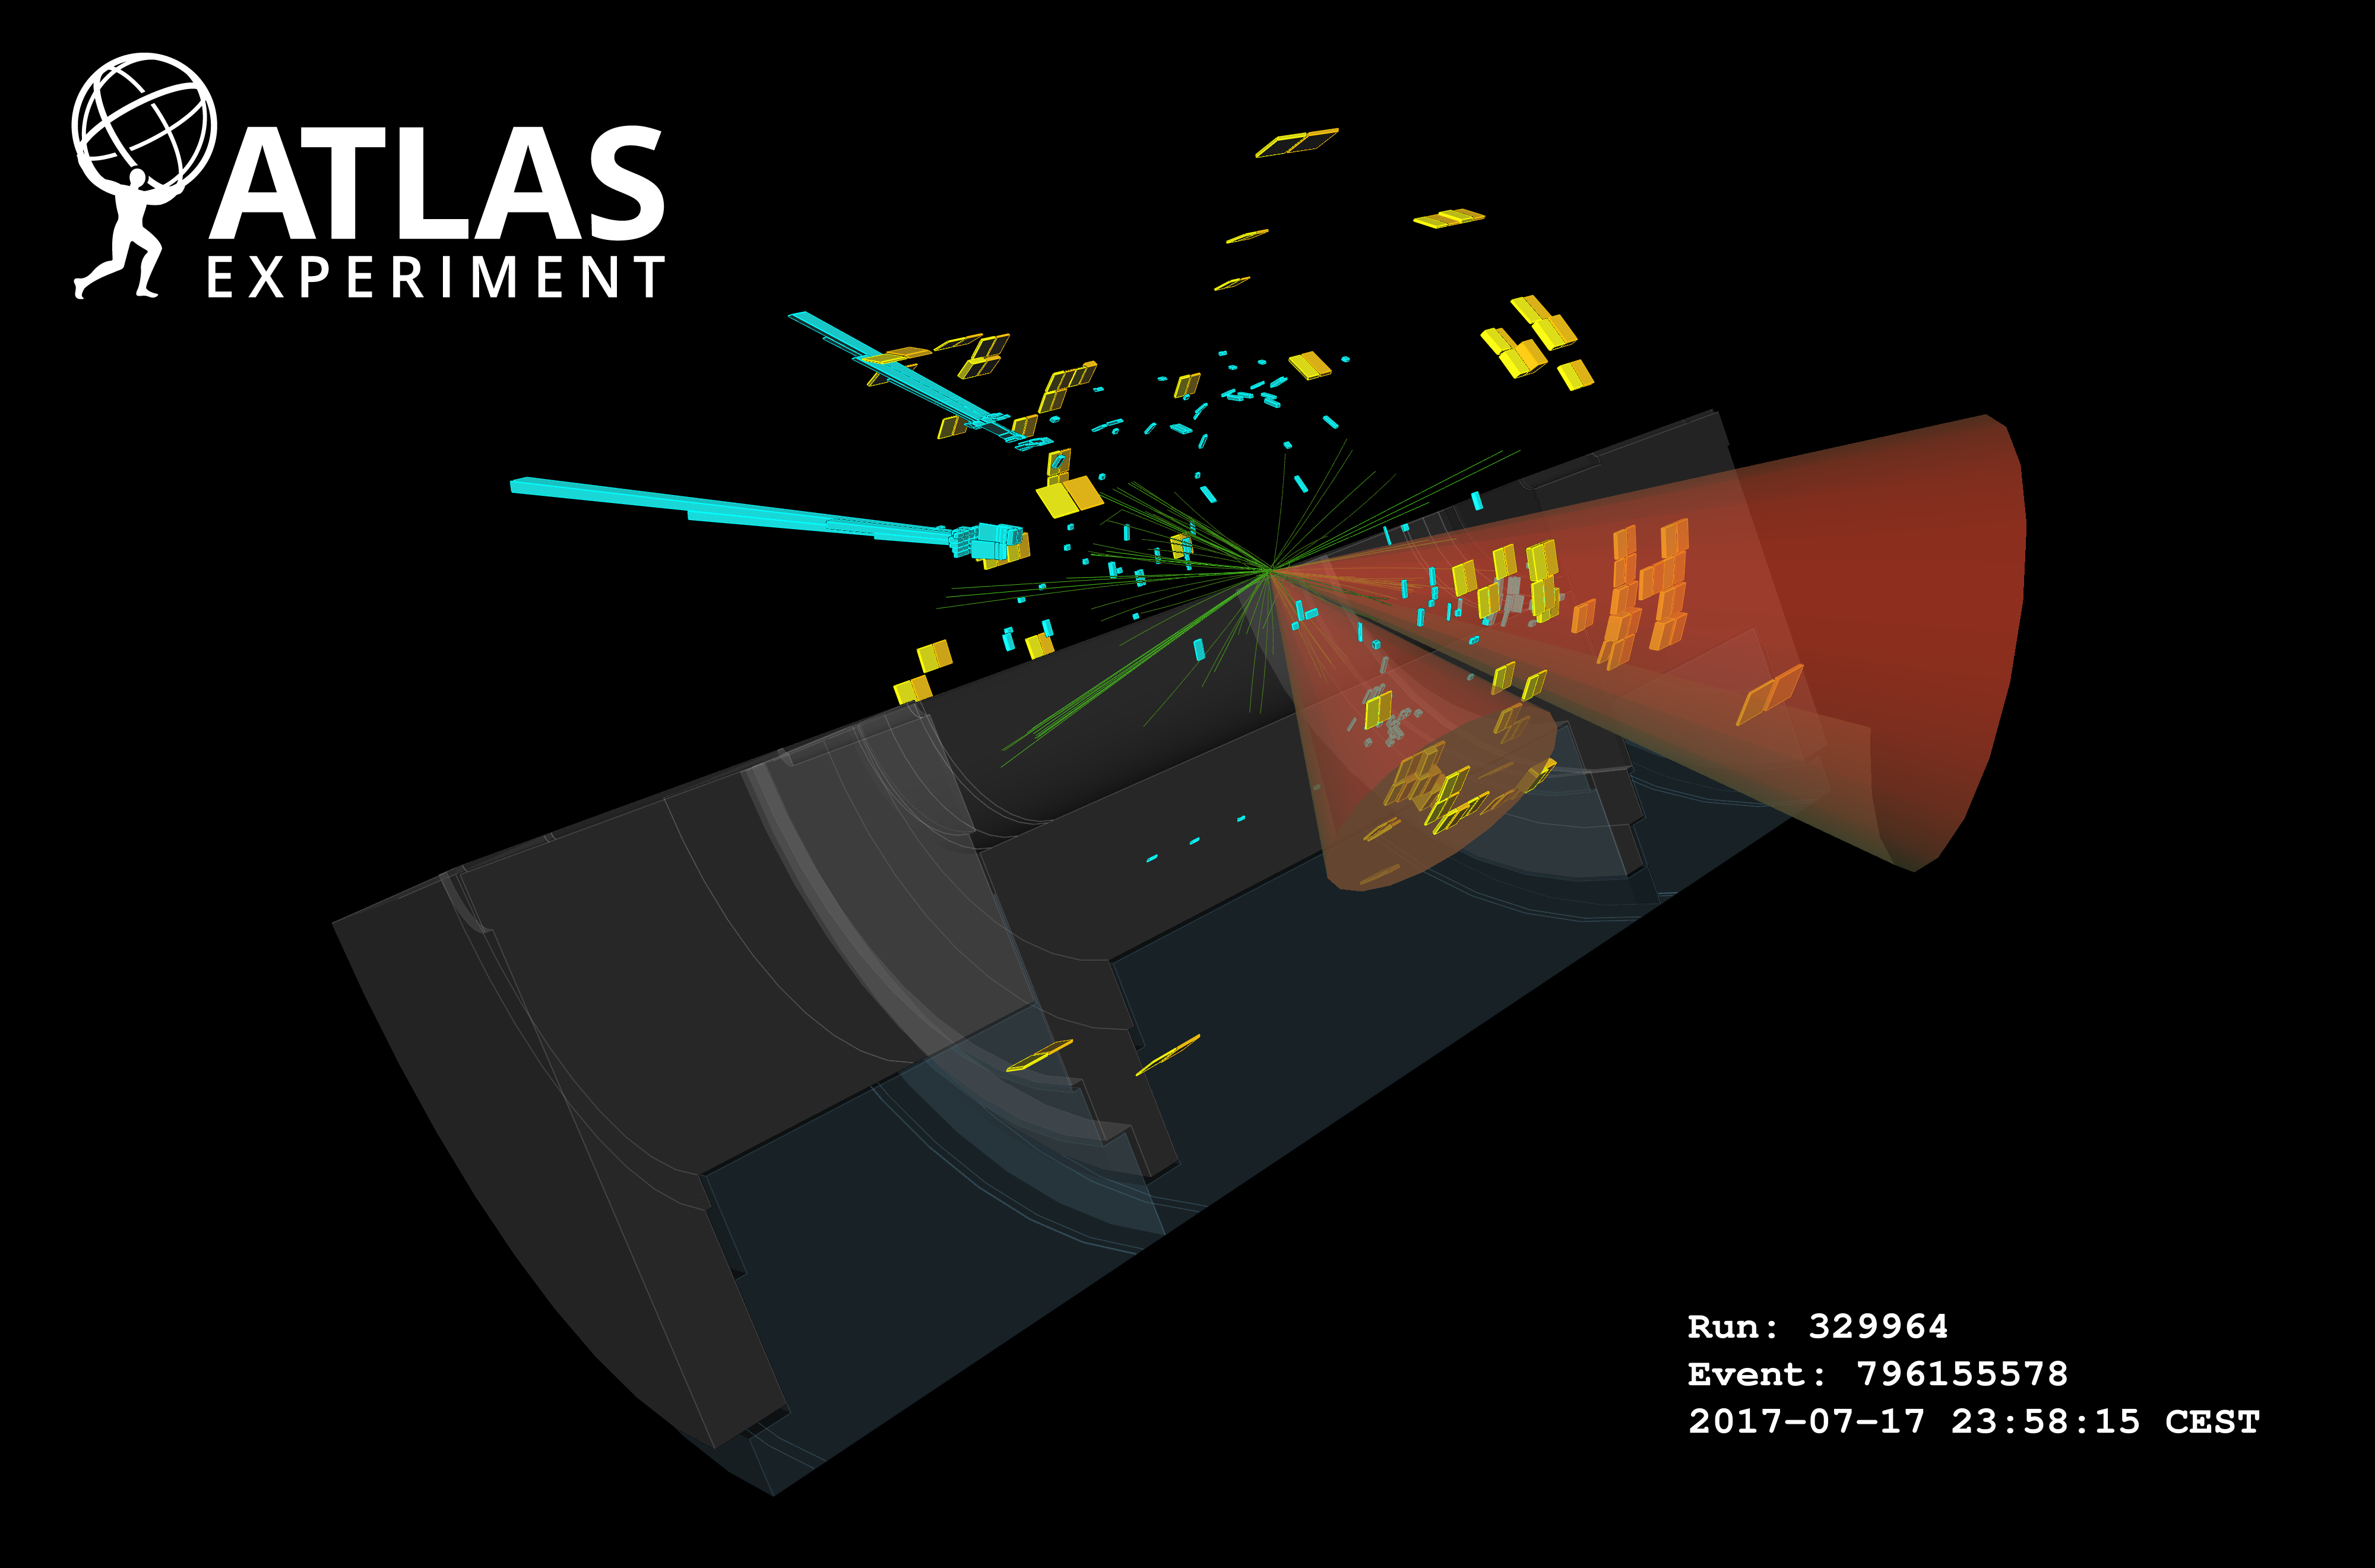
\includegraphics[width=1.03\paperwidth]{Img/figaux_01}}
\begin{frame}

\begin{textblock*}{6cm}(0.5cm,3.8cm) % {block width} (coords) 
   \textcolor{HHwhite2}{\textbf{Two narrow EM clusters $\to$ photons}}
\end{textblock*}

\begin{textblock*}{6cm}(10cm,7cm) % {block width} (coords) 
   \textcolor{HHwhite2}{\textbf{Two displaced vertices $\to$ $b$-jets}}
\end{textblock*}

\begin{textblock*}{7cm}(1cm,7cm)
 \visible<2>{% {block width} (coords) 
   \textcolor{HHwhite2}{\underline{\textbf{Backgrounds}}} \\
   \begin{itemize}
       \item \textcolor{HHwhite2}{Peaking in $m_{\gamma\gamma}$: \textbf{single H$\to\gamma\gamma$} ($t\bar{t}$H, ZH)}
       \item \textcolor{HHwhite2}{Not peaking:  \textbf{continuum $\gamma\gamma$ + jets}} 
   \end{itemize}
   }
\end{textblock*}


\end{frame}
}

\subsection{Analysis strategy}
\begin{frame}{Events selection}
\begin{columns}
\column{0.6\textwidth}

\begin{itemize}
    \item \textbf{Di-photon trigger} (83\% efficiency for HH signal)
    \begin{itemize}
        \item $E_{T}^{\gamma} > $ 35 (25) GeV for leading (sub-leading)
    \end{itemize}
    \item \textbf{$\geq $ 2 Tight} and \textbf{isolated} \textbf{photons} (\textbf{\textcolor{HHturquoise_d}{H$\to\gamma\gamma$}})
    \begin{itemize}
        \item $|\eta|< $ 2.37 \& $\frac{p_{T}^{\gamma}}{m_{\gamma\gamma}} > $ 35\% (25\%) for leading (sub-leading)
        \item $m_{\gamma\gamma}$ built with the two leading photons
    \end{itemize}
    \item \textbf{Exactly 2 $b$-jet} (\textbf{\textcolor{HHred}{H$\to b\bar{b}$}})
    \begin{itemize}
        \item $p_{T} > $ 25 GeV \& $|\eta| < $ 2.5
        \item $b$-tagging at 77\% efficiency
    \end{itemize}
    \item $<$ 6 jets, reject hadronic $t\bar{t}$H
    \item Zero leptons, reject semi-leptonic $t\bar{t}$H
\end{itemize}

\column{0.4\textwidth}

\begin{figure}
    \centering
    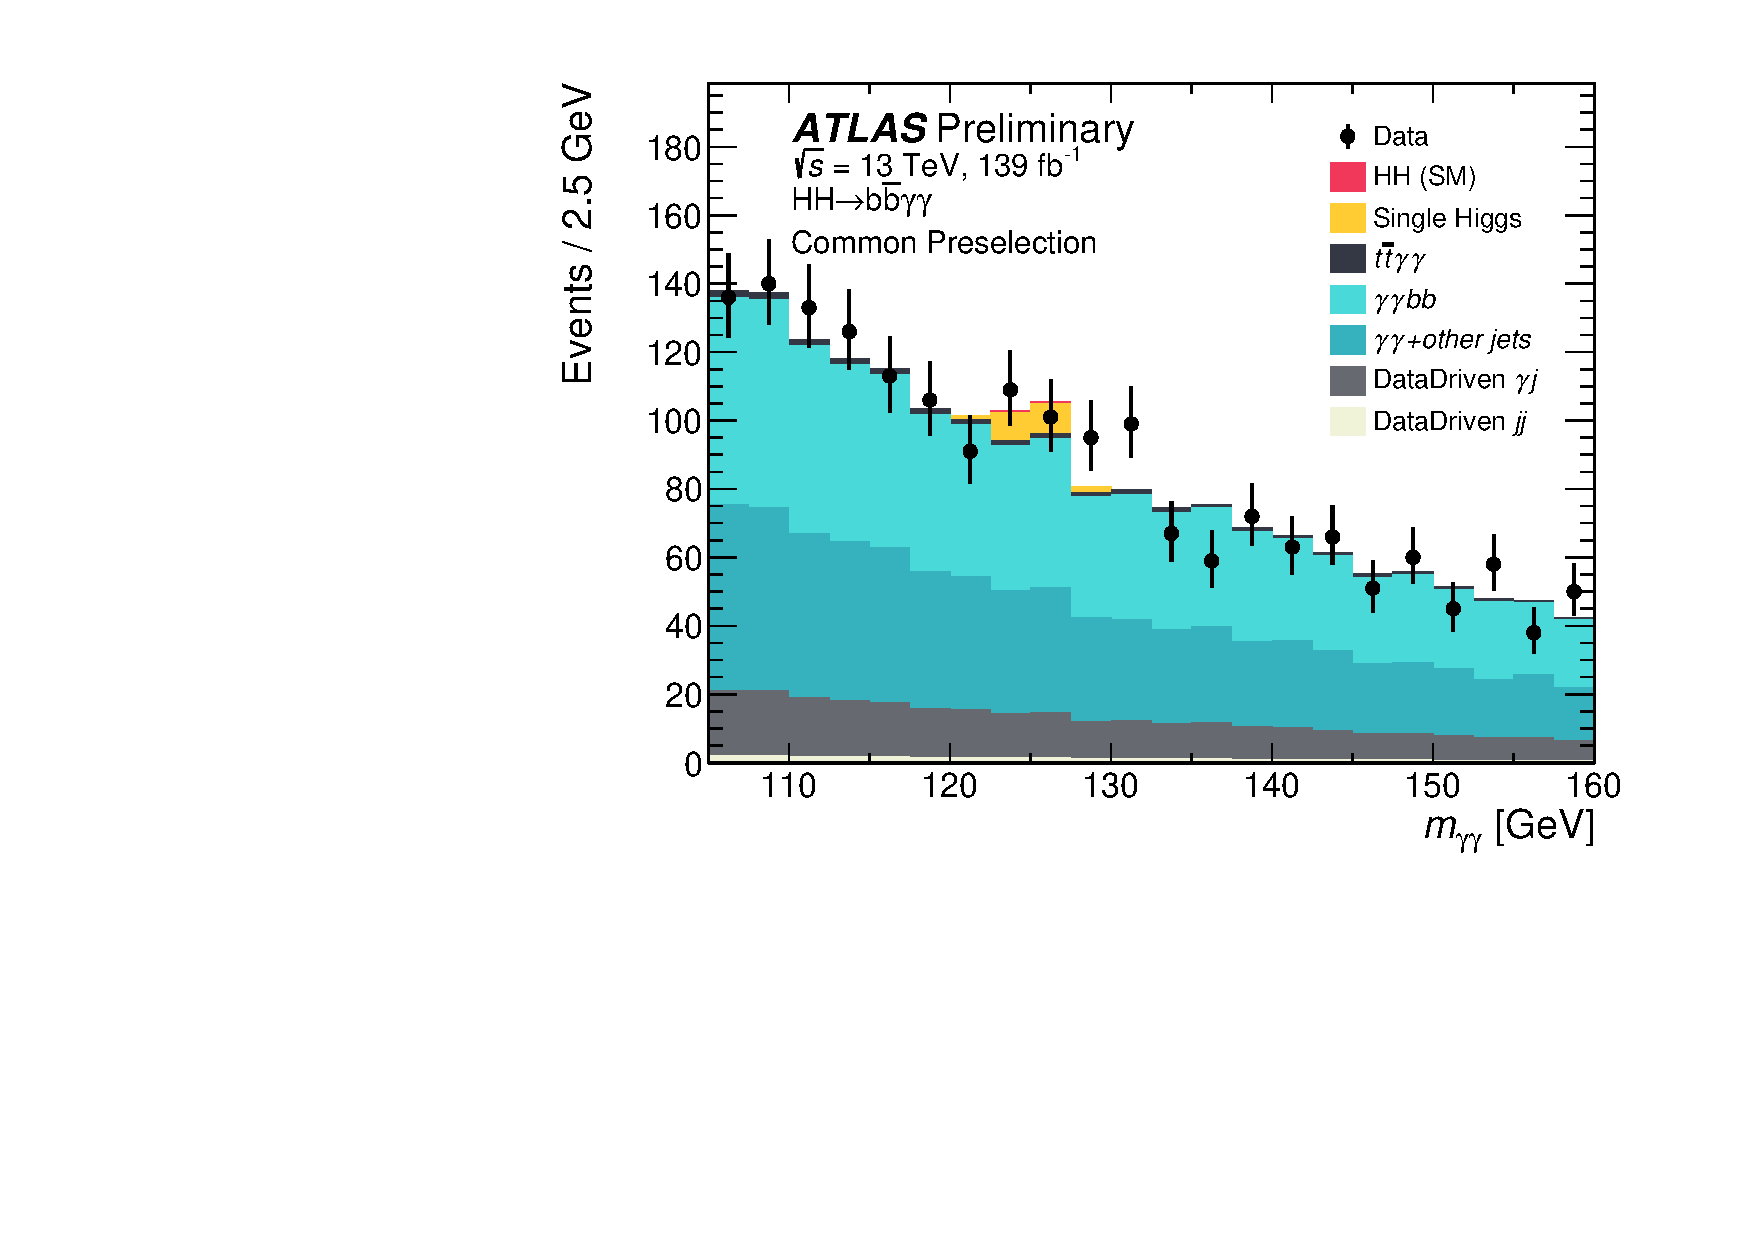
\includegraphics[width=1.1\textwidth]{Part3/Img/myy_common.pdf}
\end{figure}
\begin{center}
%\textbf{Dominant backgrounds}
%\begin{itemize}
%    \item \textbf{\textcolor{HHyellow}{Single H}} (peaking in $m_{\gamma\gamma}$): \\ \textbf{$t\bar{t}$H} + \textbf{ZH} 
%    \item \textcolor{HHturquoise_m}{\textbf{Continuum $\gamma\gamma$ + jets}}
%\end{itemize}

\end{center}
%\begin{figure}
%    \centering
%    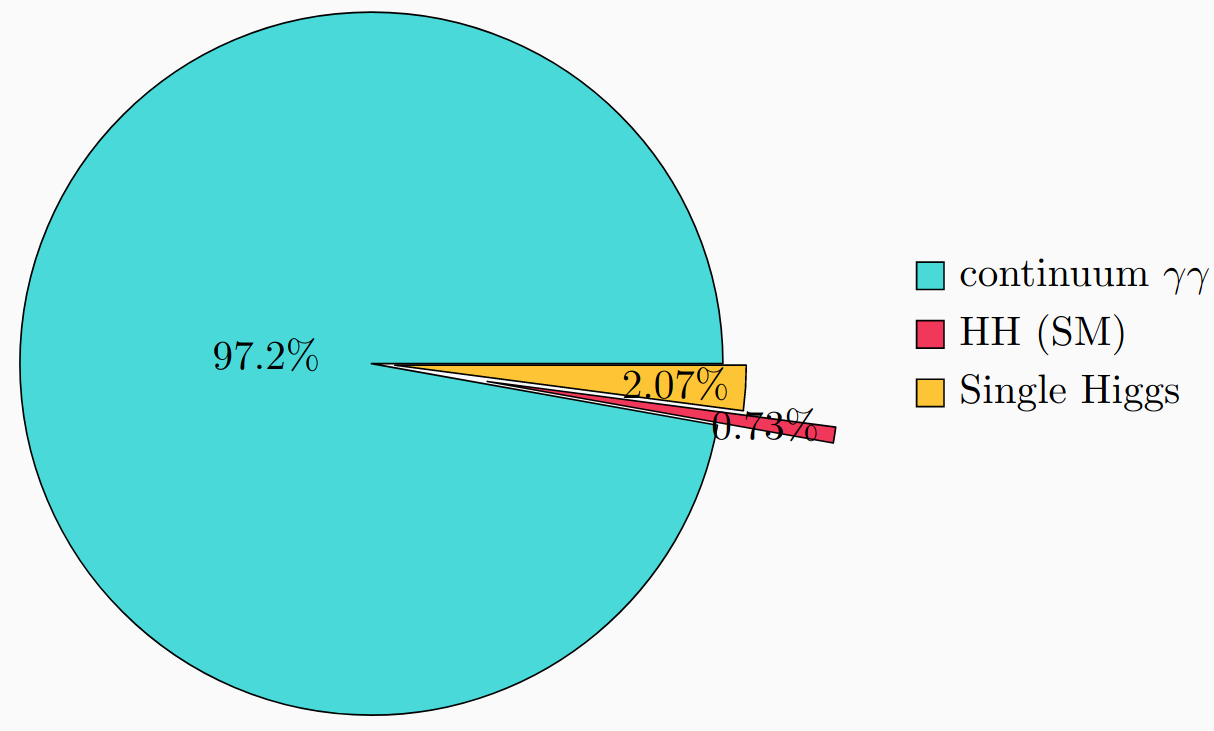
\includegraphics[width=0.7\textwidth]{Part3/Img/pie.png}
%\end{figure}

\end{columns}

\end{frame}

\begin{frame}{$b$-jet energy calibration}

\begin{textblock*}{5cm}(12cm,0.1cm) % {block width} (coords) 
   \textcolor{HHred}{\Large\textbf{my own work}}
\end{textblock*}

\begin{columns}
\column{0.4\textwidth}
\begin{figure}
    \centering
    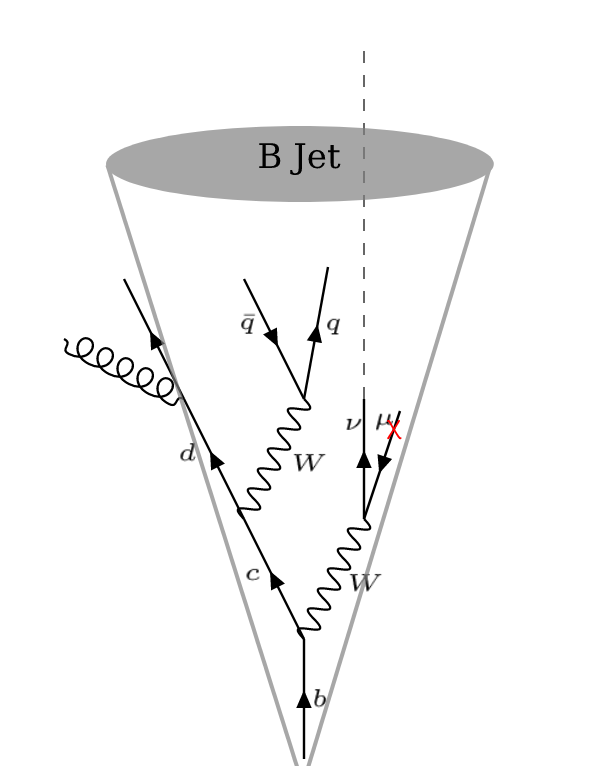
\includegraphics[width=0.8\textwidth]{Part3/Img/b-jet.png}
\end{figure}

\column{0.6\textwidth}

\begin{itemize}
    \item $m_{b\bar{b}}$ highly discriminating for H$\to b\bar{b}$
    \item $\sigma_{m_{b\bar{b}}}\sim$ 16 GeV, $\sigma_{m_{\gamma\gamma}}\sim$ 2 GeV
    \item Jets energy calibration not enough for $b$-jets,\\ due to 
    \begin{itemize}
        \item \textcolor{HHred}{\textbf{Semi-leptonic}} decay
        \item \textcolor{HHturquoise_d}{\textbf{Large $b$-quark mass}}
    \end{itemize}
\pause    
    \item Specific $b$-jet energy calibration method
    \begin{itemize}
        \item \textcolor{HHred}{\textbf{$\mu$-in-jet correction}}: presence of \textbf{muon} 
        \item \textcolor{HHturquoise_d}{\textbf{$p_T$Reco correction}}: \textbf{missing neutrino} \& \textbf{out-of-cone} radiation
    \end{itemize}
\end{itemize}
\end{columns}
\end{frame}

\begin{frame}{$b$-jet energy calibration}
\begin{textblock*}{5cm}(12cm,0.1cm) % {block width} (coords) 
   \textcolor{HHred}{\Large\textbf{my own work}}
\end{textblock*}
\begin{textblock*}{5cm}(1.9cm, 7.48cm) 
--------------------------------------
\end{textblock*}
\begin{columns}
\column{0.5\textwidth}
\begin{itemize}
    \item \textcolor{HHred}{\textbf{$\mu$-in-jet} correction}
    \begin{itemize}
        \item Adding back muons
        \item Variable $\Delta R$($b$-jet, muon) 
        \item Semi-leptonic or hadronic
    \end{itemize}
    \item \textcolor{HHturquoise_d}{\textbf{$p_T$Reco} correction}
    \begin{itemize}
        \item $p_T$-dependent scale factor
        \item Computed on \textbf{$t\bar{t}$ sample}
    \end{itemize}
\end{itemize}
\begin{figure}
    \centering
    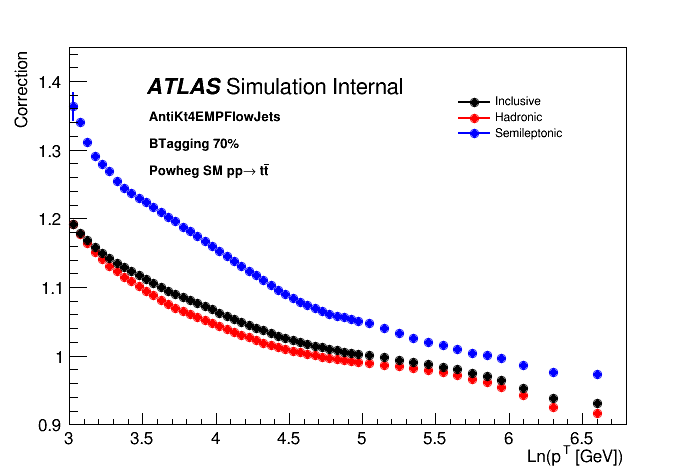
\includegraphics[width=0.8\textwidth]{Part3/Img/ptrecopflow.png}
\end{figure}

\column{0.5\textwidth}
\visible<2->{
\begin{itemize}
    \item Applied to HH$\to b\bar{b}\gamma\gamma$ $b$-jets
\end{itemize}
}
\visible<2->{
\begin{figure}
    \centering
    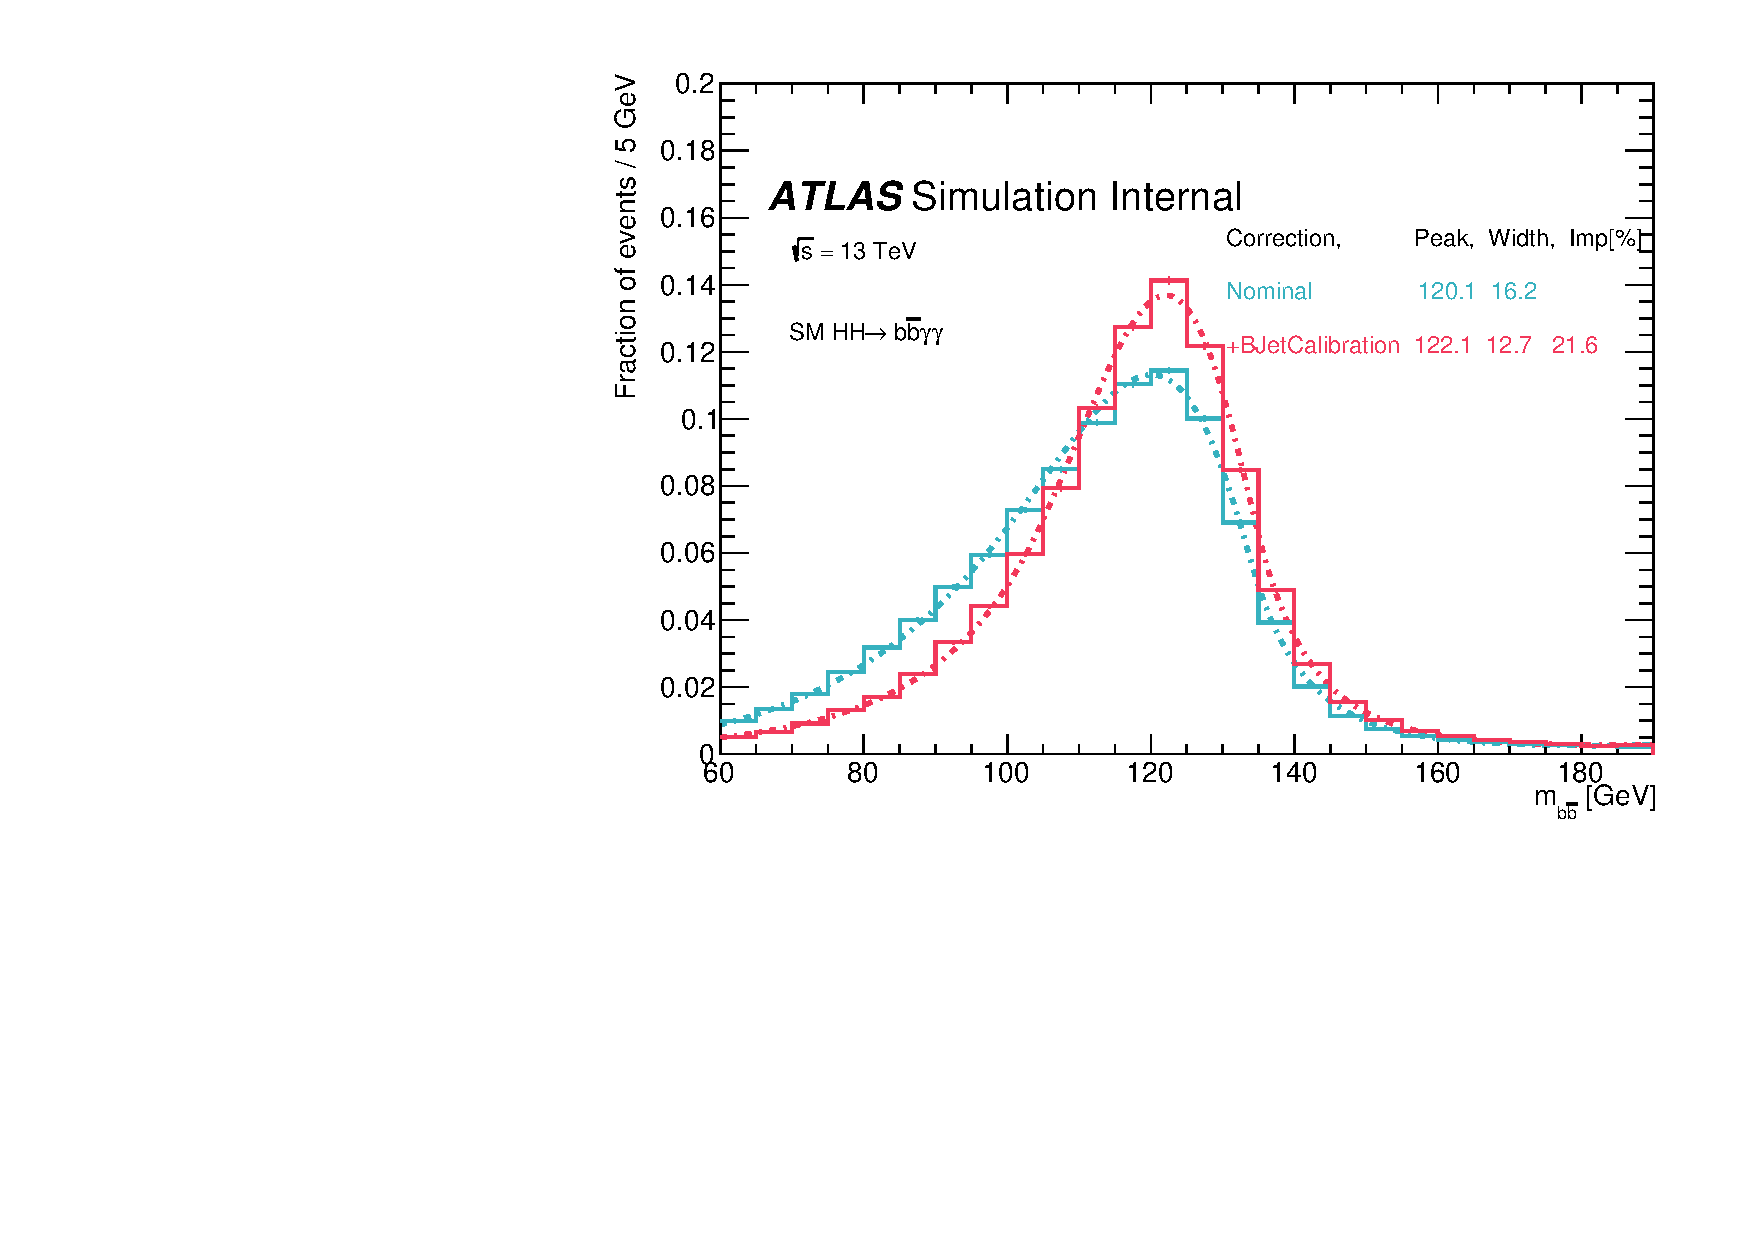
\includegraphics[width=0.9\textwidth]{Part3/Img/mbb_Paper.pdf}
\end{figure}

\begin{itemize}
    \item \textcolor{HHred}{\textbf{$\sim$22\%}} imp. on $m_{b \bar{b}}$ resolution
    \item \textcolor{HHred}{\textbf{7\% $\pm$ 2\%}} imp. on expected significance
    \item \textsl{\textbf{Baseline $b$-jet correction} for full Run-2 HH search}
\end{itemize}
}
\end{columns}    
\end{frame}


\begin{frame}{Categorization strategy}

\begin{columns}
\column{0.5\textwidth}
\begin{itemize}
    \item Sensitivity to
    \begin{itemize}
        \item \textbf{\textcolor{HHred}{SM HH signal}}
        \item \textbf{\textcolor{HHturquoise_d}{
$\kappa_{\lambda}$ deviations}}
    \end{itemize}
\pause    
    \item Two mass regions on $m_{b \bar{b}\gamma\gamma}^{*}$
    \begin{itemize}
        \item \textbf{\textcolor{HHred}{High mass} $m_{b \bar{b}\gamma\gamma}^{*} >$ 350 GeV}
        \item \textbf{\textcolor{HHturquoise_d}{Low mass} $m_{b \bar{b}\gamma\gamma}^{*} <$ 350 GeV}
    \end{itemize}
\end{itemize}

\begin{itemize}
    \item Signal-background separation: \textbf{MVA}
\end{itemize}

\column{0.5\textwidth}

\begin{textblock*}{5cm}(11cm, 3.8cm) % {block width} (coords) 
   \visible<2->{\textbf{\textcolor{HHred}{High mass}}}
\end{textblock*}
\begin{textblock*}{5cm}(9.5cm, 2.8cm) % {block width} (coords) 
   \visible<2->{\textbf{\textcolor{HHturquoise_d}{Low mass}}}
\end{textblock*}
\begin{figure}
    \begin{overprint}
    \onslide<1>\centering\centering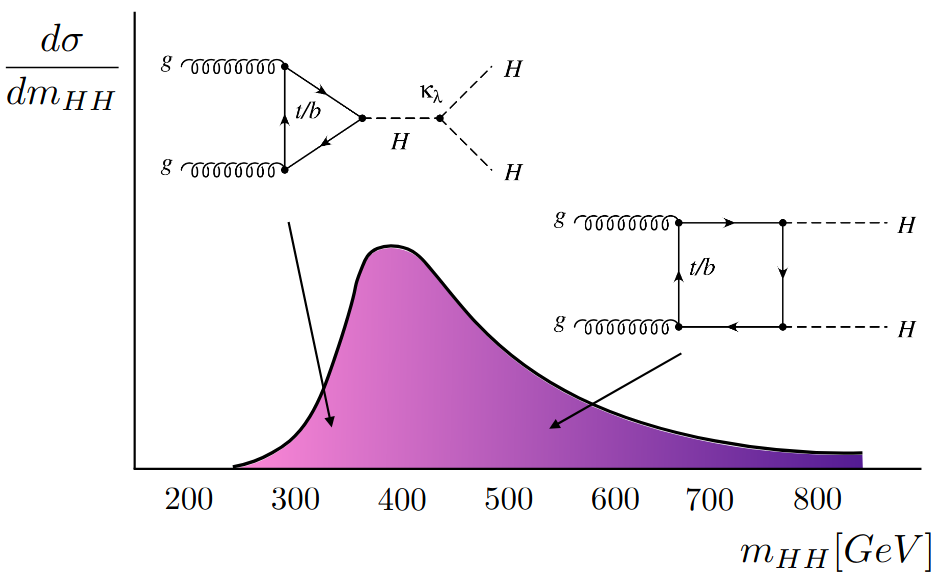
\includegraphics[width=1\textwidth]{Part3/Img/mHH_diagram2.png}
    \onslide<2->\centering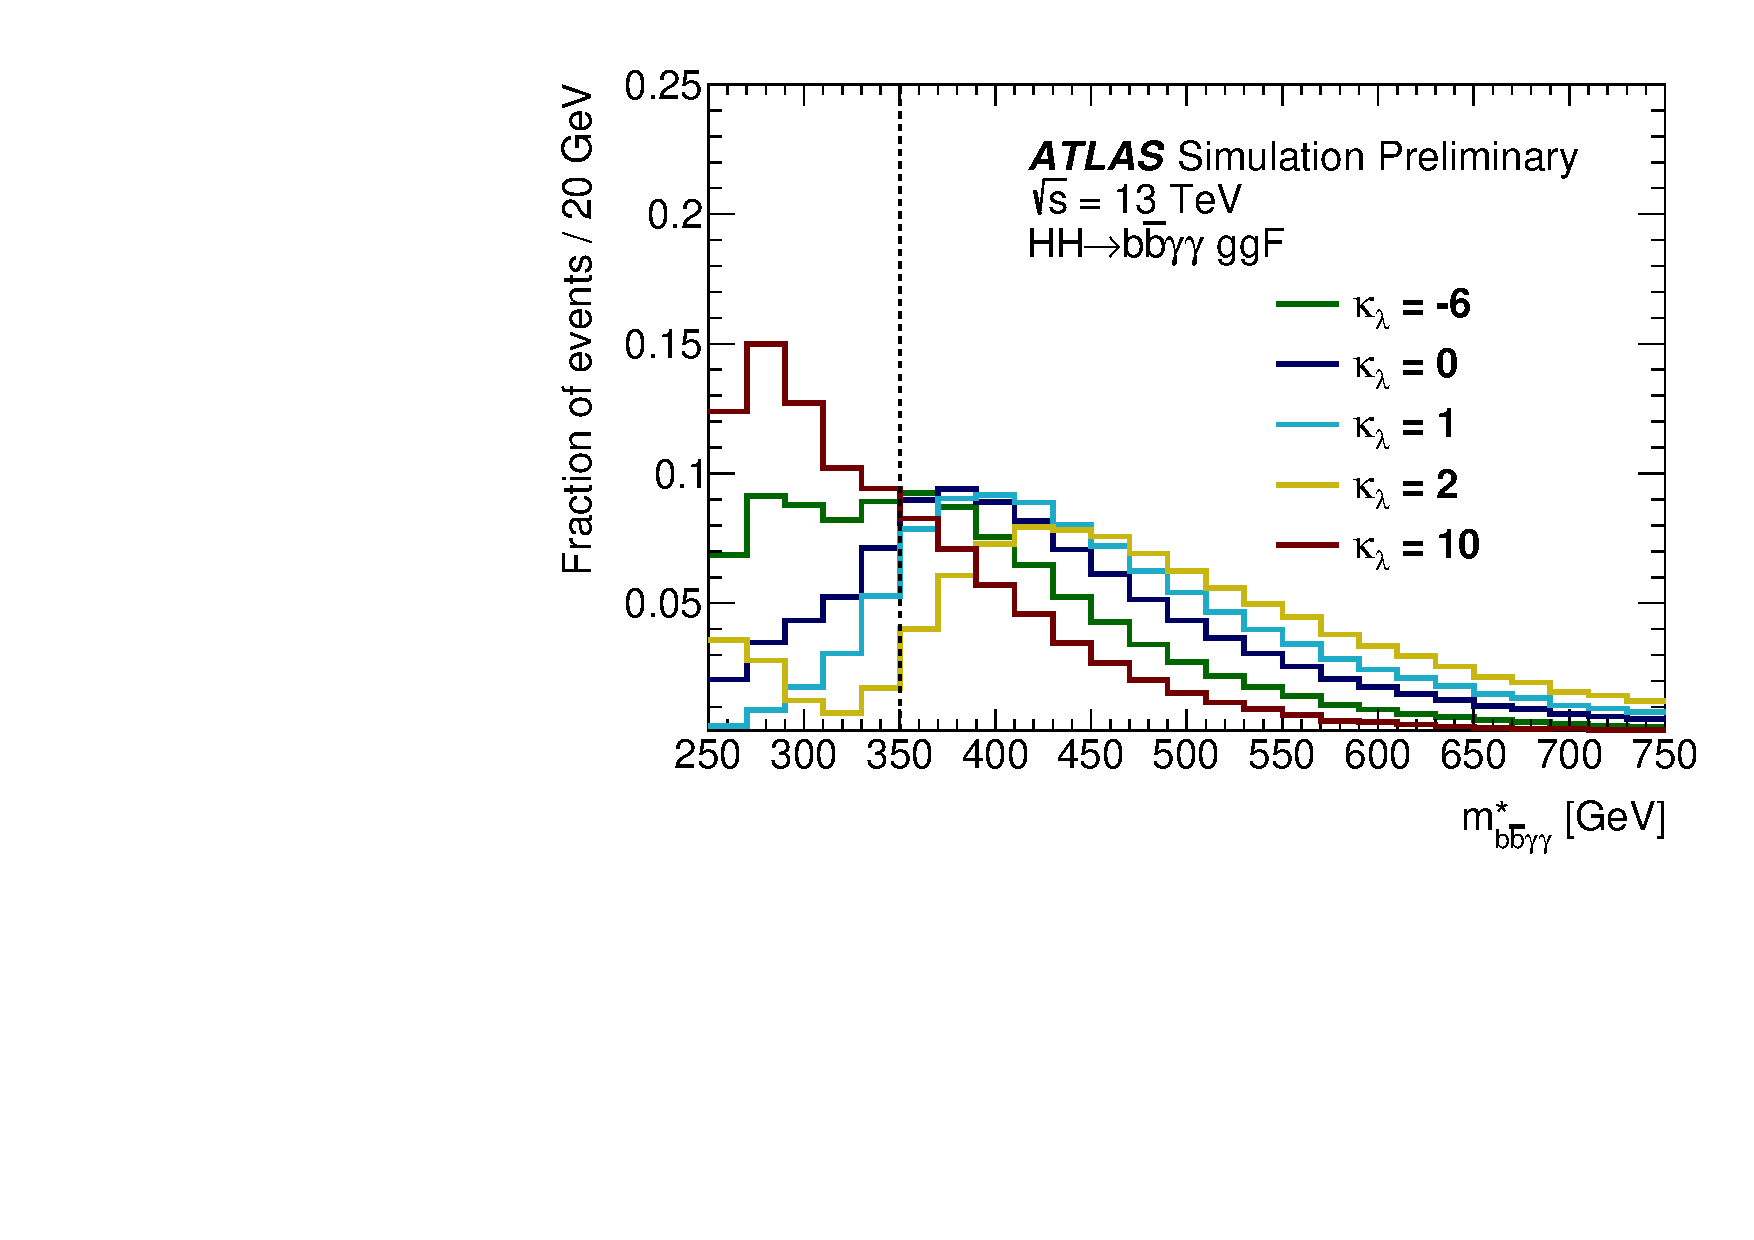
\includegraphics[width=1.1\textwidth]{Part3/Img/mbbyy_star_ggF.pdf}
    \end{overprint}
\end{figure}
\onslide<2->{
\begin{equation*}
    \textcolor{gray}{m_{b \bar{b}\gamma\gamma}^{*} =  m_{b \bar{b}\gamma\gamma} - m_{b \bar{b}} - m_{\gamma\gamma} + 250 \ \text{GeV}}
\end{equation*}
}
\end{columns}
\end{frame}

\begin{frame}{MVA categorization}

\begin{columns}
\column{0.6\textwidth}
\begin{itemize}
    \item Two MVA are trained to discriminate signal from the backgrounds
    \begin{itemize}
        \item \textbf{High mass}: \textbf{\textcolor{HHred}{SM HH ($\kappa_{\lambda} = $ 1)}}
        \item \textbf{Low mass}: \textbf{\textcolor{HHturquoise_d}{BSM HH ($\kappa_{\lambda} = $ 10)}}
    \end{itemize}
    \item Same inputs: objects and event kinematic
    \item MVA techniques
    \begin{itemize}
        \item \textcolor{structurColor}{\textbf{B}oosted \textbf{D}ecision \textbf{T}rees}: signal vs ($t\bar{t}$H + ZH + continuum $\gamma\gamma$ + jets)
        \item \textbf{D}eep \textbf{N}eural \textbf{N}etwork: signal vs $t\bar{t}$H vs ZH vs continuum $\gamma\gamma$ + jets
    \end{itemize}
\end{itemize}  

\column{0.4\textwidth}

\begin{figure}
    
    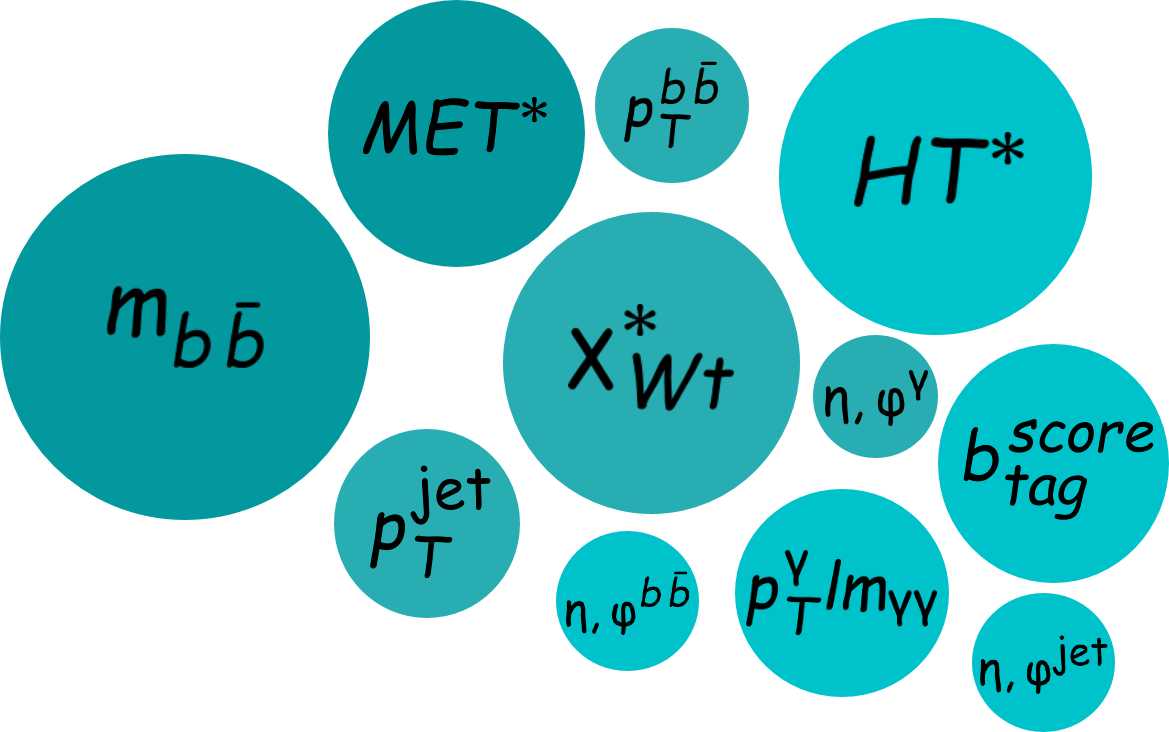
\includegraphics[width=1.\textwidth]{Part3/Img/MVA_vars.png}
\end{figure}
\textcolor{gray}{$^{*}$ not used in DNN} \\

%$\chi_{Wt}= \min \sqrt{\left(\frac{m_{j_{1} j_{2}}-m_{W}}{m_{W}}\right)^{2}+\left(\frac{m_{j_{1} j_{2} j_{3}}-m_{t}}{m_{t}}\right)^{2}}$

\end{columns}   
\end{frame}

\begin{frame}{Deep Neural Network selection}
\begin{textblock*}{5cm}(12cm,0.1cm) % {block width} (coords) 
   \textcolor{HHred}{\Large\textbf{my own work}}
\end{textblock*}
\begin{columns}
\column{0.4\textwidth}
\begin{itemize}
    \item $d_{HH}$ discriminate from 4 probabilities: 
    \begin{equation*}
        d_{HH} = \log(\frac{\sigma_{HH}.p_{HH}}{\sum^{3}{\sigma_{bkg}.p_{bkg}}})
    \end{equation*}
    \item \textbf{\textcolor{HHred}{4 categories}} maximize combined expected significance 
    \begin{itemize}
        \item \textbf{tight} and \textbf{loose} DNN for each mass region
    \end{itemize}
    \onslide<3->{
    \item \textbf{\textcolor{HHturquoise_d}{Similar performance to the BDT}}
    }
    \onslide<4->{
    \item Baseline: \textcolor{HHred}{\textbf{BDT}}
    \item \textsl{\textbf{DNN} reserved and documented for next analysis round}
    }
\end{itemize}

\column{0.6\textwidth}
\begin{textblock*}{5cm}(8.2cm, 2.4cm) % {block width} (coords) 
  \visible<1>{\rotatebox{90}{Event}}
\end{textblock*}

\begin{textblock*}{5cm}(8.5cm, 2.8cm)  
  \visible<1>{$\to$}
\end{textblock*}

\begin{textblock*}{5cm}(13.2cm, 2.3cm) 
 \visible<1>{\small \textcolor{HHturquoise_d}{HH signal}}
\end{textblock*}
\begin{textblock*}{5cm}(13.2cm, 2.6cm) % {block width} (coords) 
  \visible<1>{ \small \textcolor{HHblue}{$t\bar{t}$H}}
\end{textblock*}
\begin{textblock*}{5cm}(13.2cm, 2.9cm) % {block width} (coords) 
   \visible<1>{\small \textcolor{HHred}{ZH}}
\end{textblock*}
\begin{textblock*}{5cm}(13.2cm, 3.2cm) % {block width} (coords) 
   \visible<1>{\small \textcolor{cadmiumorange}{continuum $\gamma\gamma$+jets}}
\end{textblock*}
\begin{figure}
   \begin{overprint}
   \onslide<1>\centering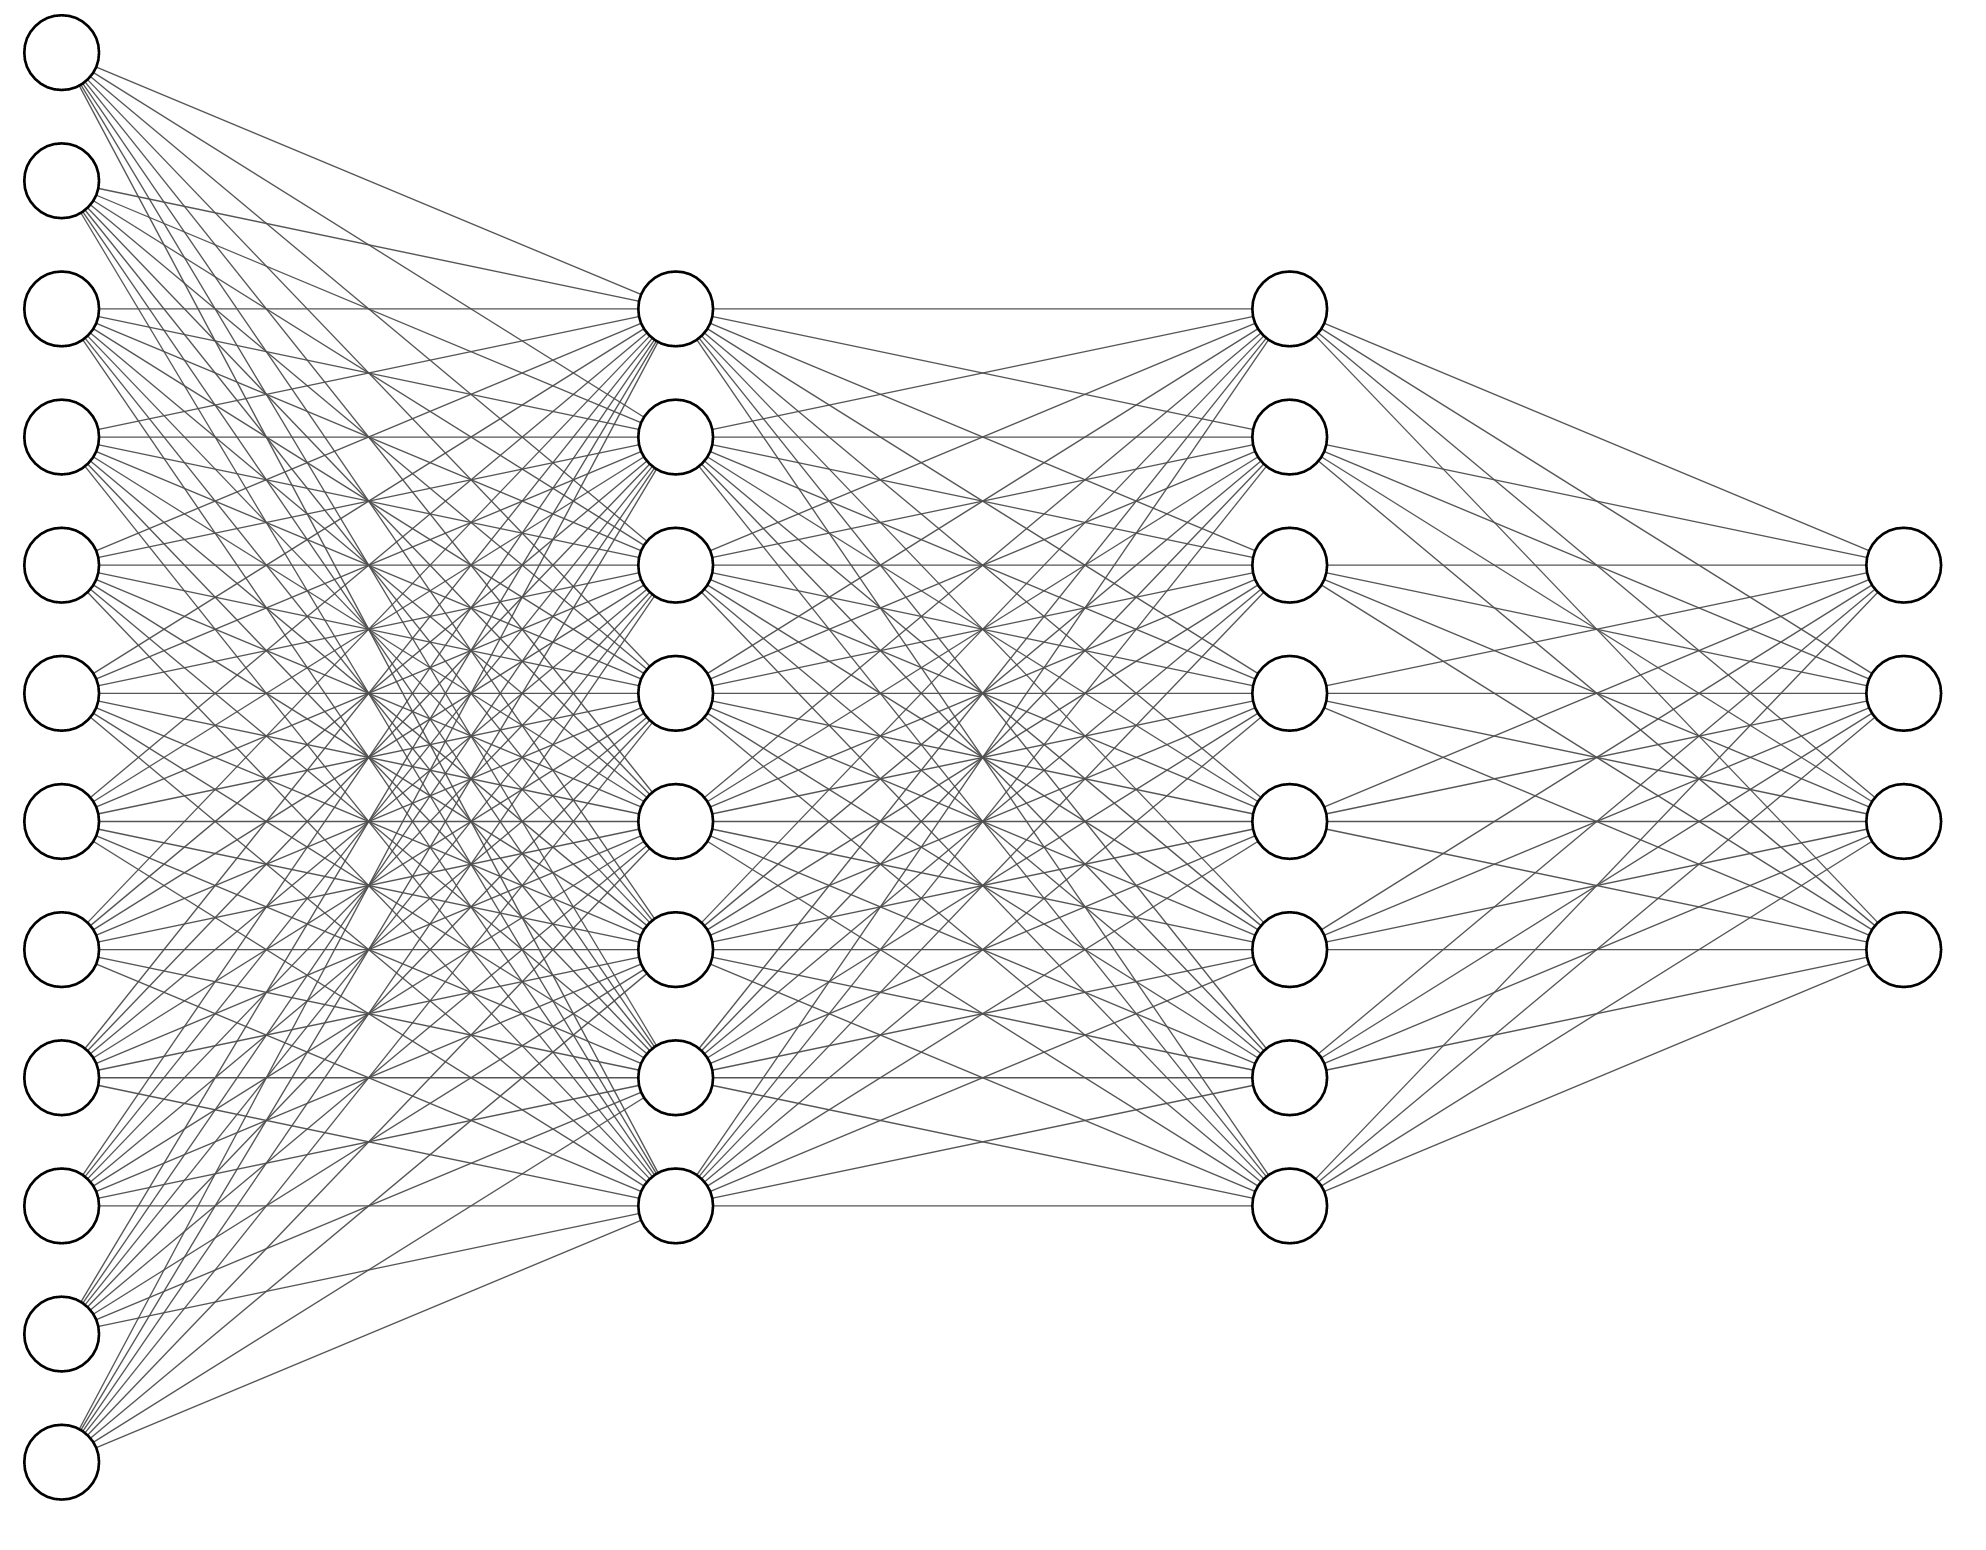
\includegraphics[width=0.5\textwidth]{Part3/Img/DNN.png}
   \onslide<2->\centering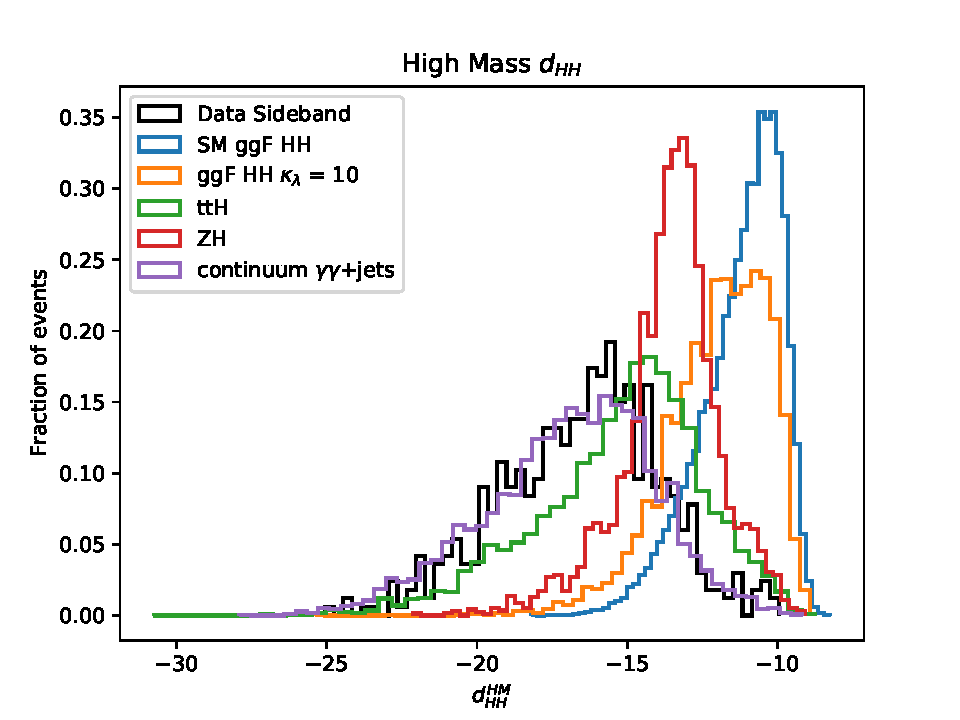
\includegraphics[width=0.7\textwidth]{Part3/Img/dHH_SM.pdf}
   \end{overprint}
 %   \subfloat{ 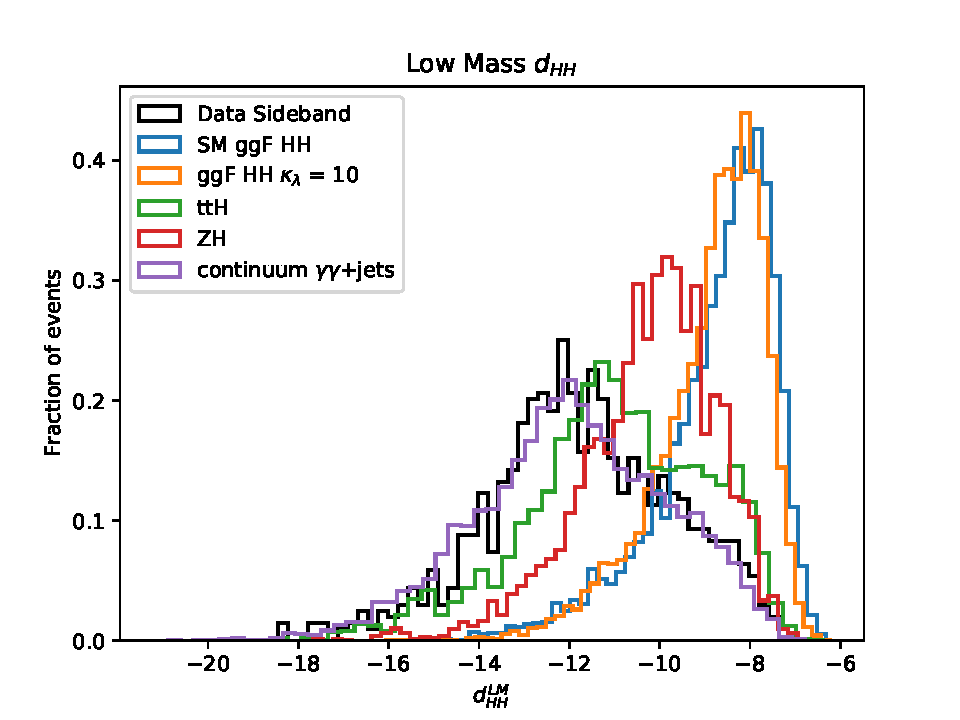
\includegraphics[width=0.55\textwidth]{Part3/Img/dHH_BSM.pdf}}
\end{figure}

\onslide<3->{
\begin{table}
    \centering
    \begin{tabular}{lcc}
    \hline\hline
        MVA & SM HH & HH $\kappa_{\lambda} = $ 10 \\
        \hline
        BDT & 0.49$\sigma$ & 3.59$\sigma$ \\
        DNN & 0.54$\sigma$ & 3.47$\sigma$ \\
        \hline\hline
    \end{tabular}
\end{table}
\begin{center}
  \textcolor{gray}{significance $ = \sqrt{2[(s+b)\times\log{(1+s/b)}-s]}$}  
\end{center}
}
\end{columns}
\end{frame}

%\begin{frame}{Signal extraction}
%\begin{columns}
%\column{0.5\textwidth}    
    
%\begin{itemize}
%    \item \textcolor{HHturquoise_d}{$m_{\gamma\gamma}$ modelling in the 4 analysis categories}
%    \item \textbf{\textcolor{red}{HH signal} (ggF + VBF)}: 
%    \begin{itemize}
%        \item \textbf{from Monte Carlo}
%        \item \textbf{Yield parametrized as a function of $\kappa_{\lambda}$}
%        \item Double-sided Crystal-Ball (DSCB)
%    \end{itemize}
%    \item \textbf{\textcolor{red}{Single Higgs}}: 
%    \begin{itemize}
%        \item \textbf{from Monte Carlo}
%        \item Same PDF as the signal (injection test)
%    \end{itemize}
%    \item \textbf{\textcolor{blue}{Continuum $\gamma\gamma$}}:
%    \begin{itemize}
%        \item \textbf{fully data driven}
%        \item smoothly falling analytic function 
%        \item Spurious signal test: quantify model bias $\to$ systematic uncertainty
%    \end{itemize}
%\end{itemize}    
%    
%\column{0.5\textwidth}
%\begin{figure}
%    \centering
%    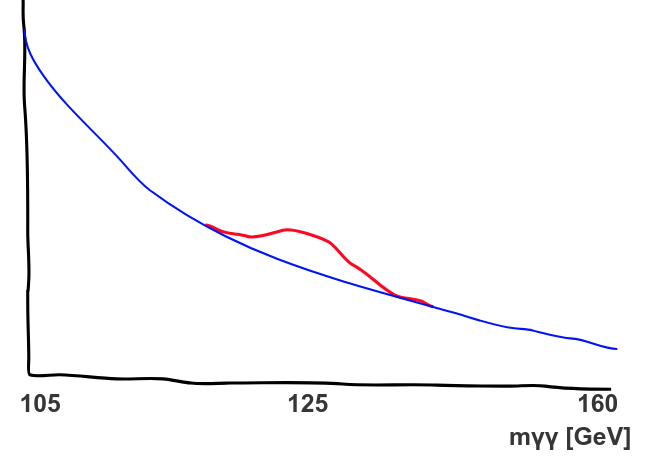
\includegraphics[width=0.8\textwidth]{Part3/Img/myysketch.png}
%\end{figure}
%\end{columns}
%    
%\end{frame}

\subsection{Higgs self-coupling constrain}

\begin{frame}{Signal extraction and results}

\begin{columns}
\column{0.6\textwidth}
\begin{itemize}
    \item Simultaneous fit of \textbf{$m_{\gamma\gamma}$} in the 4 analysis categories
    \begin{itemize}
        \item \textbf{\textcolor{HHred}{HH signal} (ggF + VBF) + \textcolor{HHred}{Single Higgs}}
        \begin{itemize}
            \item \textbf{from Monte Carlo} using Double-sided Crystal-Ball
        \end{itemize}
       \item \textbf{\textcolor{HHturquoise_d}{Continuum $\gamma\gamma$ + jets}}
       \begin{itemize}
           \item \textbf{fully data driven}
       \end{itemize}
    \end{itemize}
    \item \textbf{\textcolor{HHred}{No significant signal is observed}}
    \item 95\% CL upper limits on $\sigma_{ggF+VBF}$ of diHiggs as a function of $\kappa_{\lambda}$
\end{itemize}

\column{0.4\textwidth}
\begin{textblock*}{5cm}(13.3cm, 3.6cm) % {block width} (coords) 
   \textbf{\textcolor{HHred}{--------------}}
\end{textblock*}
\begin{figure}
    \centering
    \fcolorbox{gray}{HHwhite2}{
    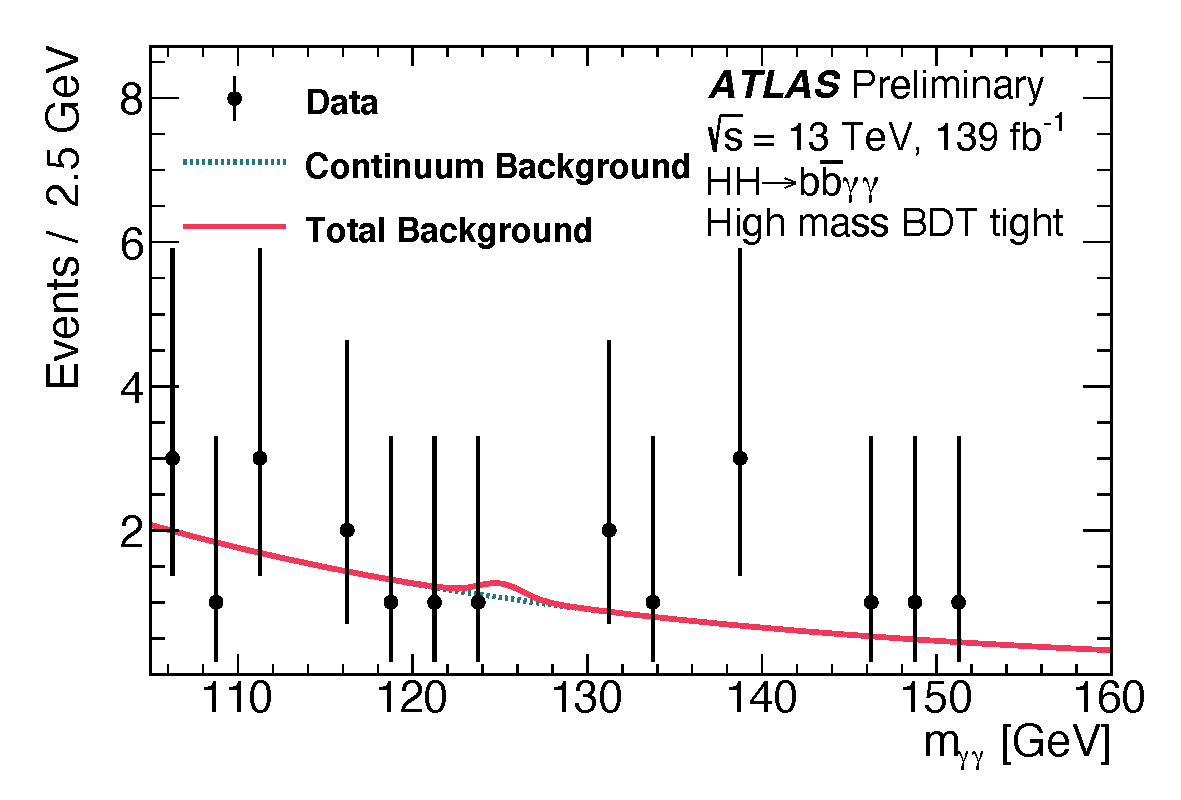
\includegraphics[width=1.\textwidth]{Part3/Img/myy_bkg_only_high_mass_tight_BDT.pdf}
    }
\end{figure}

\begin{center}
   \textcolor{gray}{ \textbf{most sensitive category}}
\end{center}

\end{columns}    
\end{frame}


\begin{frame}{Limits and $\kappa_{\lambda}$ constrain}
\setbeamercovered{transparent}
\begin{columns}
\column{0.4\textwidth}

\begin{textblock*}{5cm}(2cm,2.2cm) % {block width} (coords) 
   \textcolor{HHred}{\textbf{\href{https://atlas.web.cern.ch/Atlas/GROUPS/PHYSICS/CONFNOTES/ATLAS-CONF-2021-016}{ATLAS-CONF-2021-016}}}
\end{textblock*}

\begin{textblock*}{6cm}(8cm,4.5cm) % {block width} (coords) 
  \visible<2>{ \textcolor{HHred}{\Large\textbf{The world's best $\kappa_{\lambda}$ limit}}}
\end{textblock*}

\begin{figure}
    \centering
    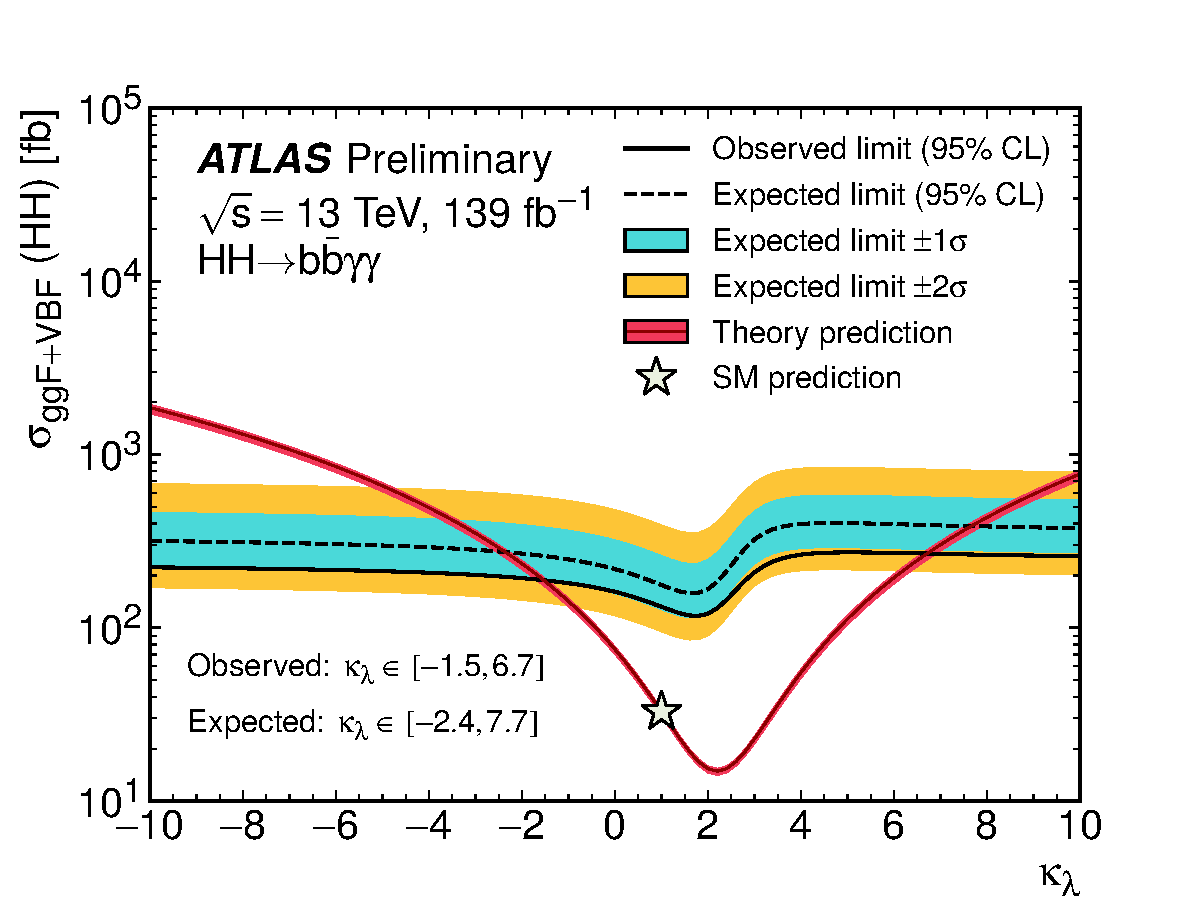
\includegraphics[width=1.1\textwidth]{Part3/Img/limit_yybb.pdf}
\end{figure}

\column{0.6\textwidth}

\begin{itemize}
    \item $\frac{\sigma_{HH}}{\sigma_{HH}^{SM}}$ limit: \textbf{\textcolor{HHred}{4.1}} (Exp. \textbf{5.5}) at 95\% CL
    \item $\kappa_{\lambda}$ constrain: \textbf{\textcolor{HHred}{[-1.5, 6.7]}} (Exp. \textbf{[-2.4, 7.7]})
    \onslide<3->{
    \item \textbf{Statistically limited}
    \begin{itemize}
        \item Systematic effect $\sim$ \textbf{4\%}
        \item Background modelling \& photon energy scale
    \end{itemize}
    }
    \onslide<4->{
    \pause
    \item \textbf{\textcolor{cadmiumorange}{5$\times$ improvement}} w.r.t 36 fb$^{-1}$
    \begin{itemize}
        \item Increased luminosity: 2$\times$
        \item \textbf{\textcolor{HHturquoise_d}{Analysis improvement: almost 3$\times$}}
        \begin{itemize}
            \item$m_{HH}$ categorization and MVA strategy (\textbf{80\%})
            \item $b$-jet energy calibration (\textbf{7\%})
            \item ...
        \end{itemize}
    \end{itemize}
    }
  %  \item HH$\to b\bar{b}\tau^+\tau^-$ $\frac{\sigma_{HH}}{\sigma_{HH}^{SM}}$ limit: \textcolor{HHred}{\textbf{4.7}} (Exp. \textbf{3.9})
\end{itemize}
\end{columns}
\end{frame}

\begin{frame}{CMS HH$\to b\bar{b}\gamma\gamma$ results}

\begin{columns}
\column{0.5\textwidth}

\begin{textblock*}{5cm}(2cm,2.2cm) % {block width} (coords) 
   \textcolor{HHred}{\textbf{\href{https://doi.org/10.1007/JHEP03(2021)257}{ JHEP03 (2021) 257}}}
\end{textblock*}

\begin{itemize}

    \item \textbf{\textcolor{structurColor}{Different analysis strategies}}
    \begin{itemize}
        \item 14 categories
        \begin{itemize}
            \item \textbf{MVAs output} and \textbf{$m_{b\bar{b}\gamma\gamma}^{*}$}
            \item \textbf{2 dedicated VBF categories} 
        \end{itemize}
        \item \textcolor{HHturquoise_d}{\textbf{2D fit}} $m_{\gamma\gamma}\times m_{b\bar{b}}$
    \end{itemize}
\end{itemize}

\column{0.5\textwidth}

\begin{table}[]
    \centering
    \begin{tabular}{lcc}
    \hline\hline
    & Expected & Observed \\
    \hline 
    CMS $\frac{\sigma_{HH}}{\sigma_{HH}^{SM}}$ limit & \textbf{5.2} & 7.7 \\
    CMS $\kappa_{\lambda}$ interval & \textbf{[-2.5, 8.2]} & [-3.3, 8.5] \\
    \hline 
    ATLAS $\frac{\sigma_{HH}}{\sigma_{HH}^{SM}}$ limit & \textbf{5.5} & 4.1 \\
    ATLAS $\kappa_{\lambda}$ interval & \textcolor{HHred}{\textbf{[-2.4, 7.7]}} & [-1.5, 6.7] \\ 
    \hline\hline
    \end{tabular}
    
\end{table}

%\begin{figure}
    %\centering
    %\fcolorbox{HHturquoise_d}{HHwhite2}{
    %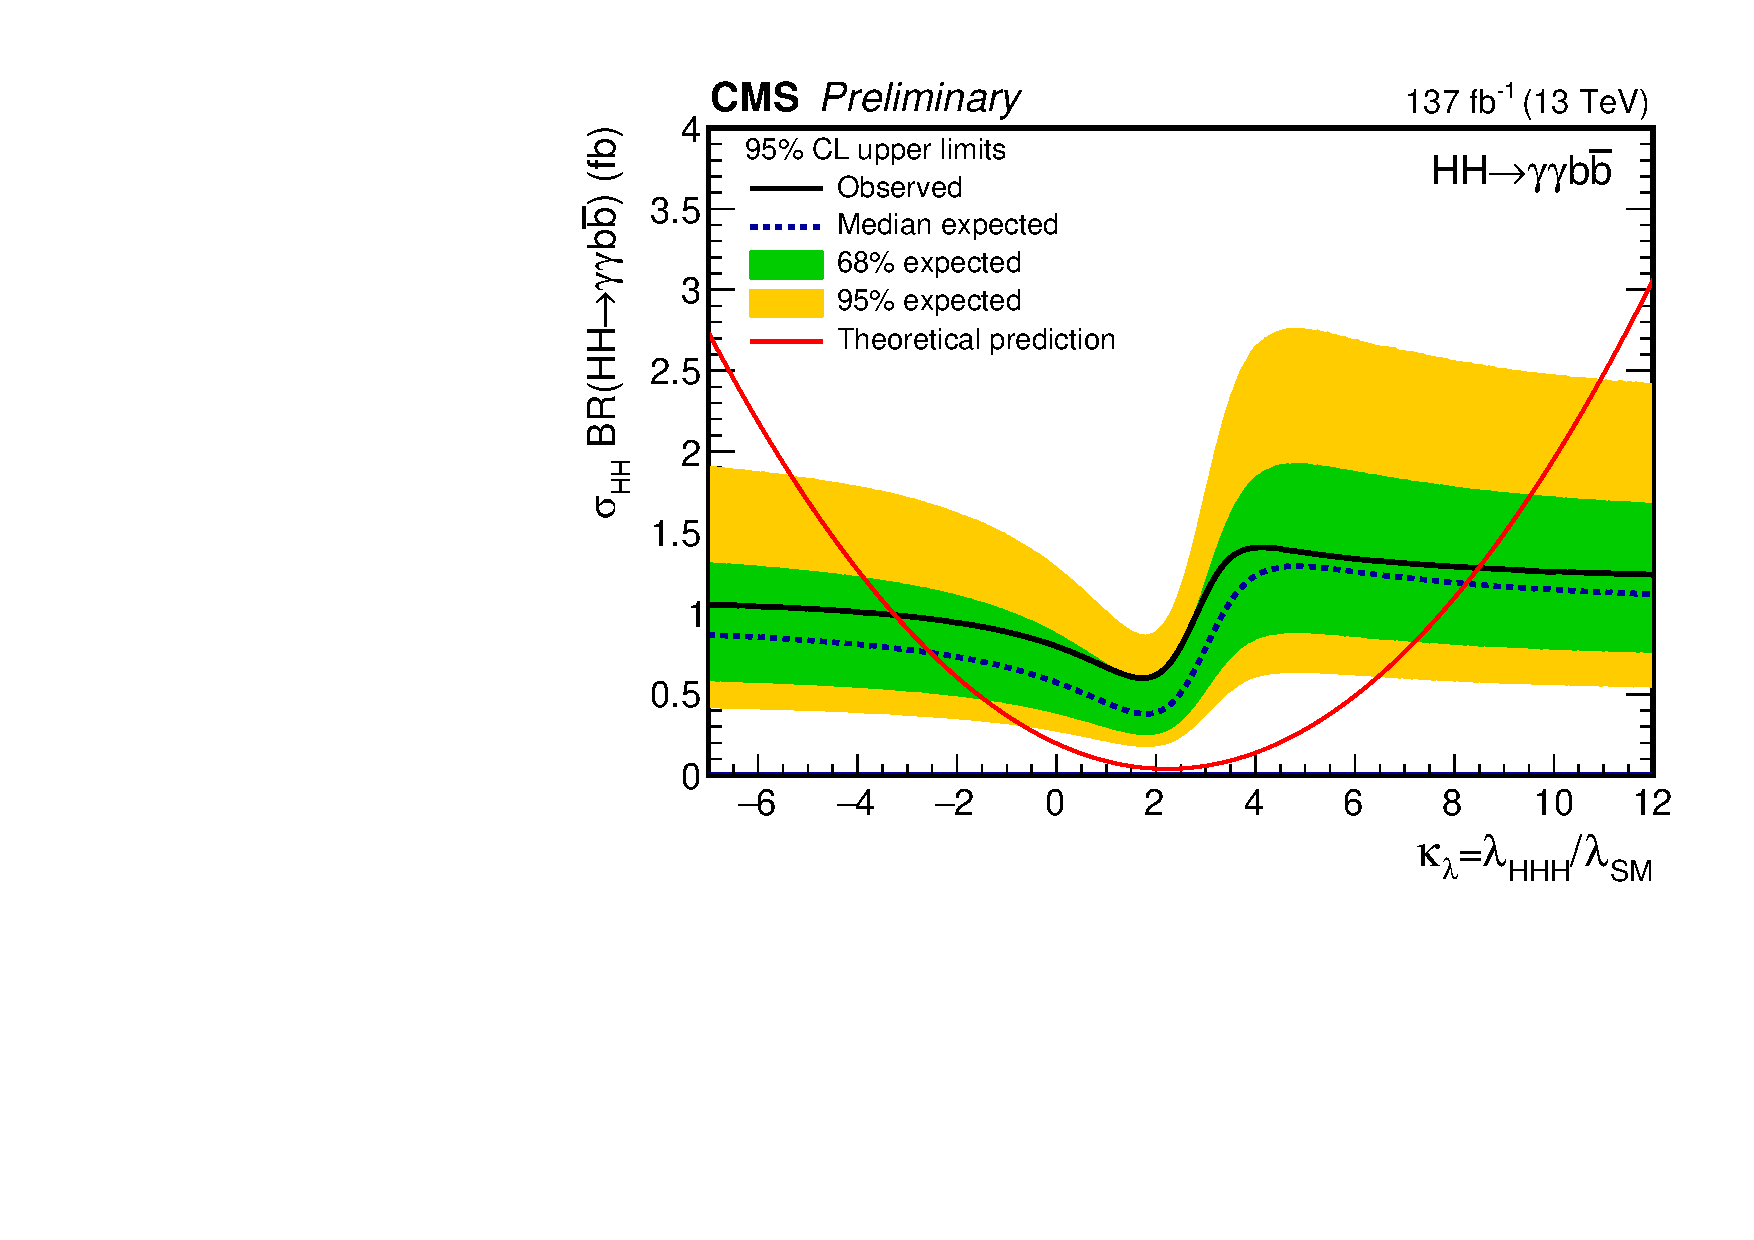
\includegraphics[width=1.\textwidth]{Part3/Img/CMS_kl_scan.pdf}
    %}
%\end{figure}
\end{columns}
\end{frame}

